---
title: "Flexplot: Graphically-Based Data Analysis"
author: "Dustin Fife"
date: "`r Sys.Date()`"
output: rmarkdown::html_vignette
vignette: >
  %\VignetteIndexEntry{Flexplot: Graphically-Based Data Analysis}
  %\VignetteEngine{knitr::rmarkdown}
  %\usepackage[utf8]{inputenc}
bibliography: references2.bib
---


```{r, echo=FALSE, message=FALSE, warning=FALSE}
library(knitr)
# set global chunk options
#opts_chunk$set(prompt=TRUE)
#options(replace.assign=TRUE, width = 90, prompt = "Rzan> ")
```


# Introduction

In light of the recent "replication crisis" in science [@Pashler2012a; @open_science_collaboration_estimating_2015], researchers are becoming increasingly concerned with the validity of science [@Baker2016a]. As such, many are pushing for greater transparency and reproducibility [@Nelson2018; @Nosek2018]. One way to accomplish greater transparency is through abudant use of data visualizations [@Tay2016a], particularly when data are presented in their raw form. 

In addition to answering the call for greater transparency, graphics offer several additional advantages. First, they improve communication between the scientific community and the public [@Otten2015]. Lay people can understand relatively sophisticated statistical procedures when that information is presented graphically [@Correll2015]. Additionally, graphics highlight problems with models that are masked by traditional statistical procedures, such as nonlinearity, outliers, and heteroscedasticity [@Healy2014a; @Levine2018]. As such, graphics serve as an important diagnostic check. Finally, graphics improve encoding [@Hansen]. Consider the image displayed in Figure \ref{fig:smiley}, taken from \cite{Correll2015}. The table on the left presents the same information as the one on the right, though the encoding of the information on the right is much easier because that information is conveyed *visually.*


<!-- \begin{figure}[t!] -->
<!-- \label{fig:smiley} -->
<!-- \centering -->
<!-- 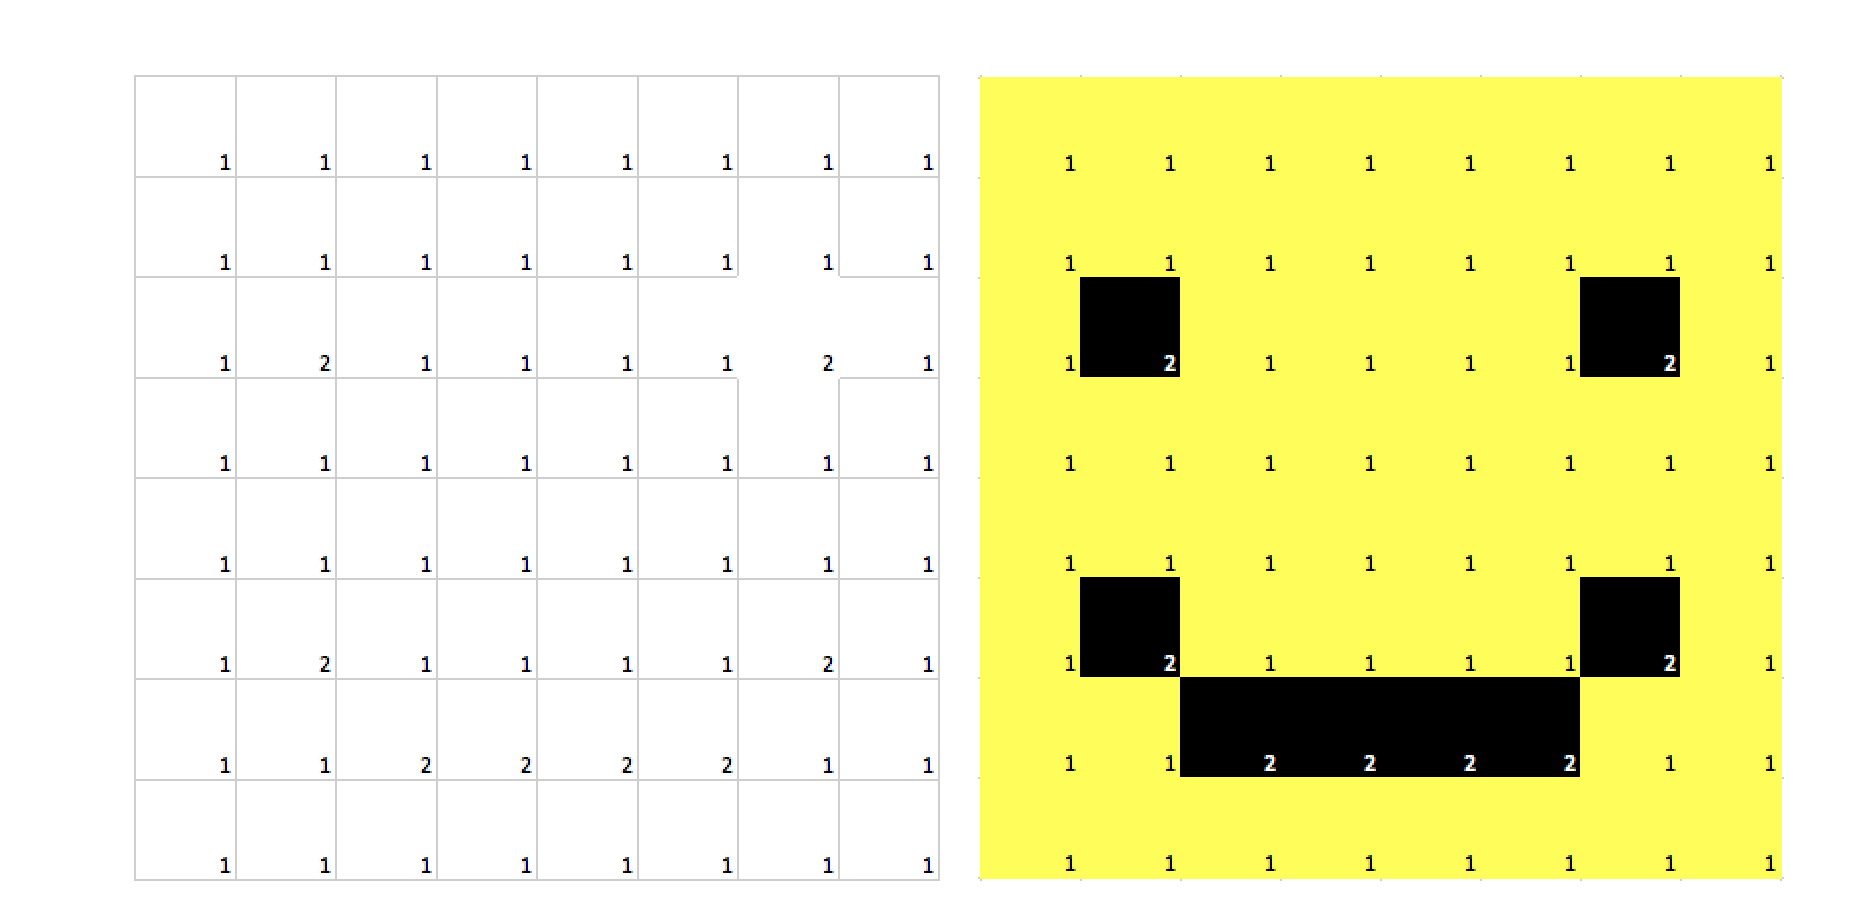
\includegraphics[width = 14cm]{images/smiley.png} -->
<!-- \caption{A table of numbers on the left, and a color-coded table on the right, where the 1's have been highlighted in yellow and the 2's in black. With the color, a pattern emerges that was not easy to see without the graphic. Figure used with permission from \cite{Correll2015}.} -->
<!-- \end{figure} -->

```{r, smiley, out.width = "400px", fig.cap = "A table of numbers on the left, and a color-coded table on the right, where the 2's have been highlighted in yellow. With the color, a pattern emerges that was not easy to see without the graphic. Figure used with permission from Correll (2015). \\label{fig:smiley}", message=FALSE, warning=FALSE,fig.align='center'}
require(ggplot2)
require(flexplot)
data(exercise_data)
knitr::include_graphics("images/smiley.png")
```


```{r, message=FALSE, warning=FALSE, echo=FALSE, fig.align = 'center'}
require(ggplot2)
require(flexplot)
data(exercise_data)
```



While visualizations have many advantages, they can also be used to mislead, sometimes intentionally, and sometimes not. For example, when means/standard errors are presented as barcharts, people tend to judge values below the mean (i.e., within the confines of the bar) as far more likely than values above the mean, even when the underlying distribution is symmetric [@Correll2015]. To further complicate matters, the default images in most point-and-click statistical software violate important visualization heuristics [@Fife2019d]. For example, in \proglang{SPSS} it is impossible (as far as I know) to produce standard error plots that display raw data (jittered or otherwise). Also, in standard error plots, the axes are scaled to the means, not the range of the actual data, which visually inflates the size of the effect. In addition, producing some types of graphics (e.g., Skew-Location plots) require more effort than many are willing to perform (the user must model the data, export the residuals, then produce a scatterplot).

\pkg{flexplot} was designed to address these limitations. It was developed using empirically-derived heurstics that maximize perceptual understanding, while minimizing perceptual biases [@Fife2019d]. Also, the graphics produced are simple to generate and permit analysts to quickly shift between statistical modeling and graphical interpretation. 


# Existing graphical software
This package builds upon \pkg{ggplot2} [@Wickham2011b] and aims to convert \proglang{R} models to graphics. Other packages are designed to do similar things. For example, \pkg{visreg} [@Breheny]  also offers one-line functions for models, though lacks some of the tools unique to \pkg{flexplot} (such as ghost lines and advanced customization of how variables are visualized). Furthermore, it doesn't allow one to visually compare models like \pkg{flexplot} does and \pkg{visreg} can only visualize a smaller subset of variables than \pkg{flexplot} can. \pkg{ggfortify} [@Tang2016] also offers the ability to visualize fitted models, but focuses on clustering and time series analyses. Finally, \pkg{tourr} [@Wickham2011], like \pkg{flexplot}, offers multivariate visualizations through tours of multivariate data, but these are animated graphics, which can only be reproduced in a limited number of environments. No other package, that I know of, was derived using principles of human factors and visual processing. 


<!-- \subsection[Guiding philosophy of flexplot]{Guiding philosophy of \pkg{flexplot}} \label{sec:philosophy} -->
# Guiding philosophy of flexplot

The design of \pkg{flexplot} is based on the following principles: 

*1. Minimize obstacles to producing graphics.* The easier it is to produce graphics, the more likely they will be used, and the more resources the researcher will have available to interpret the results. Technology companies spend millions of dollars attempting to make the interaction between humans and technology as seamless as possible. One-click purchasing, voice-activated personal assistants like Siri, movies-on-demand, and audible app notifications are all innovations that are successful because they make it easy to use their technology. Likewise, if producing a graphic is as simple (or simpler) than performing a statistical analysis, they too will become heavily utilized (and, dare I say, addictive?) Furthermore, the less effort required to produce them, the more resources available to invest in *interpreting* graphics. To make producing graphics as simple as possible, \pkg{flexplot} automates much of the decision-making in the background, such as choosing between types of graphics (e.g., histograms versus bar charts) and how those graphics are displayed.

*2. Design graphics that leverage human strenths and mitigate human biases.* Successful technology capitalizes on human strengths. A mobile phone, for example, leverages our advanced finger tactile sensitivity and dexterity. Sending text messages with a one's toes would be a very poor choice. Likewise, a computer that sends olefactory information might work well for a dog, but not a human. Visualization technology ought to be designed with the same principles in mind. Unfortunately, standard statistical analyses do not capitalize on human strengths. It takes a great deal of training to understand even basic statistics, and even then results are frequently misinterpreted [@Gigerenzer2004]. To overcome miconceptions about statistical analyses, some of the tools within \pkg{flexplot} create visual representation of the statistical models. These representations highlight uncertainty, reveal whether chosen models are appropriate, and improve encoding of statistical information. 

# A new grammar of graphics
Hadley Wickham, the author of \pkg{ggplot2}, developed a "layered" grammar of graphics [@Wickham2010]. Wickham's grammar allows a great deal flexibility in the design of graphics. However, this flexibility comes at cost. Very often the grammar necessary to produce a graphic requires a great deal of coding to produce. For example, consider the code to create jittered mean plots:


```{r, message=FALSE, echo=TRUE, warning=FALSE, options(prompt=" ", continue=" ")}
plot = ggplot(data = exercise_data, aes(x=therapy.type, y=weight.loss)) +
  geom_jitter(width = .2, alpha = .4) +
  stat_summary(fun.y = 'mean', geom = 'point', 
        size = 3, position = position_dodge(width = .2)) +
  stat_summary(geom = 'errorbar', fun.ymin = function(z){mean(z)-1.96*sd(z)}, 
        fun.ymax=function(z) {mean(z)+1.96*sd(z)}, 
        size = 1.25, width = .2, position = position_dodge(width = .2)) 
```
As noted earlier, the more difficult it is to produce a graphic, the more likely it is someone will simply not use it. A similar graphic can be produced with only one line of code using the `flexplot()` function:

```{r, message=FALSE, echo=TRUE, warning=FALSE}
plot = flexplot(weight.loss ~ therapy.type, data = exercise_data)
```


Naturally, this simplicity comes at a cost; \pkg{flexplot} is more limited than \pkg{ggplot2}. However, it was not designed to be able to produce any graphic conceivable. Rather it was designed to visualize statistical models with ease, and will cover the majority of graphics analysts will use for modeling. However, in the end, graphics produced through \pkg{flexplot} are still \pkg{ggplot2} objects. As such, they can be edited and/or layered for further customization, which I will demonstrate throughout this paper. 


\pkg{flexplot}'s grammar is also a layered grammar (but incidentally, because it developed within \pkg{ggplot2}'s grammar), though its grammar is actually based on the general linear model (GLM). Recall that most statistical procedures are subsumed within the GLM, which is essentially regression. For example, a t-test is simply a regression where the intercept is the mean of the referent group (e.g., the control group) and the slope is simply the difference between the treatment and control groups. The base \proglang{R} function \code{lm} utilizes GLMs to do various sorts of modeling, and all this is accomplished using a simple equation (e.g., `y ~ x1 + x2`). Likewise, \pkg{flexplot} adopts the same convention, utilizing a similar equation to produce graphics. Figure \ref{fig:flexplotgrammar} is an illustration that identifies which components of a \pkg{flexplot} equation produce each element of a \pkg{flexplot}-style graphic. The first variable in the equation ($X1$) specifies which variable is displayed on the $X$ axis. The second variable ($X2$) is displayed as different colors/symbols/lines. The third and fourth elements are shown as column and row panels, respectively. By following the grammar of a GLM, there is consistency between statistical modeling and visualization, with a few notable exceptions. Most obviously, a GLM equation (e.g., `plot(y ~ x1 + x2 + x3, data = data)`) does not have any vertical pipes (`|`) as `flexplot()` does. This is necessary in `flexplot()` to allow more specificity in paneling. Additionally, with GLMs, one must explicitly specify interaction (e.g., `X1:X2`) and polynomial terms (e.g., `I(X2^2)`). This is not necessary with `flexplot()`; the raw data are displayed exactly as they are and if interactions are present, the visual will show it. 


<!-- \begin{figure}[h] -->
<!-- \caption{A diagram showing how elements of \pkg{flexplot}'s graphics are represented in a plot. $X1$ is shown on the $X$ axis, $X2$ shows up as different colors/symbols/lines, $X3$ panels in columns, and $X4$ panels in rows.} -->
<!-- \label{fig:flexplotgrammar} -->
<!-- \centering -->
<!-- 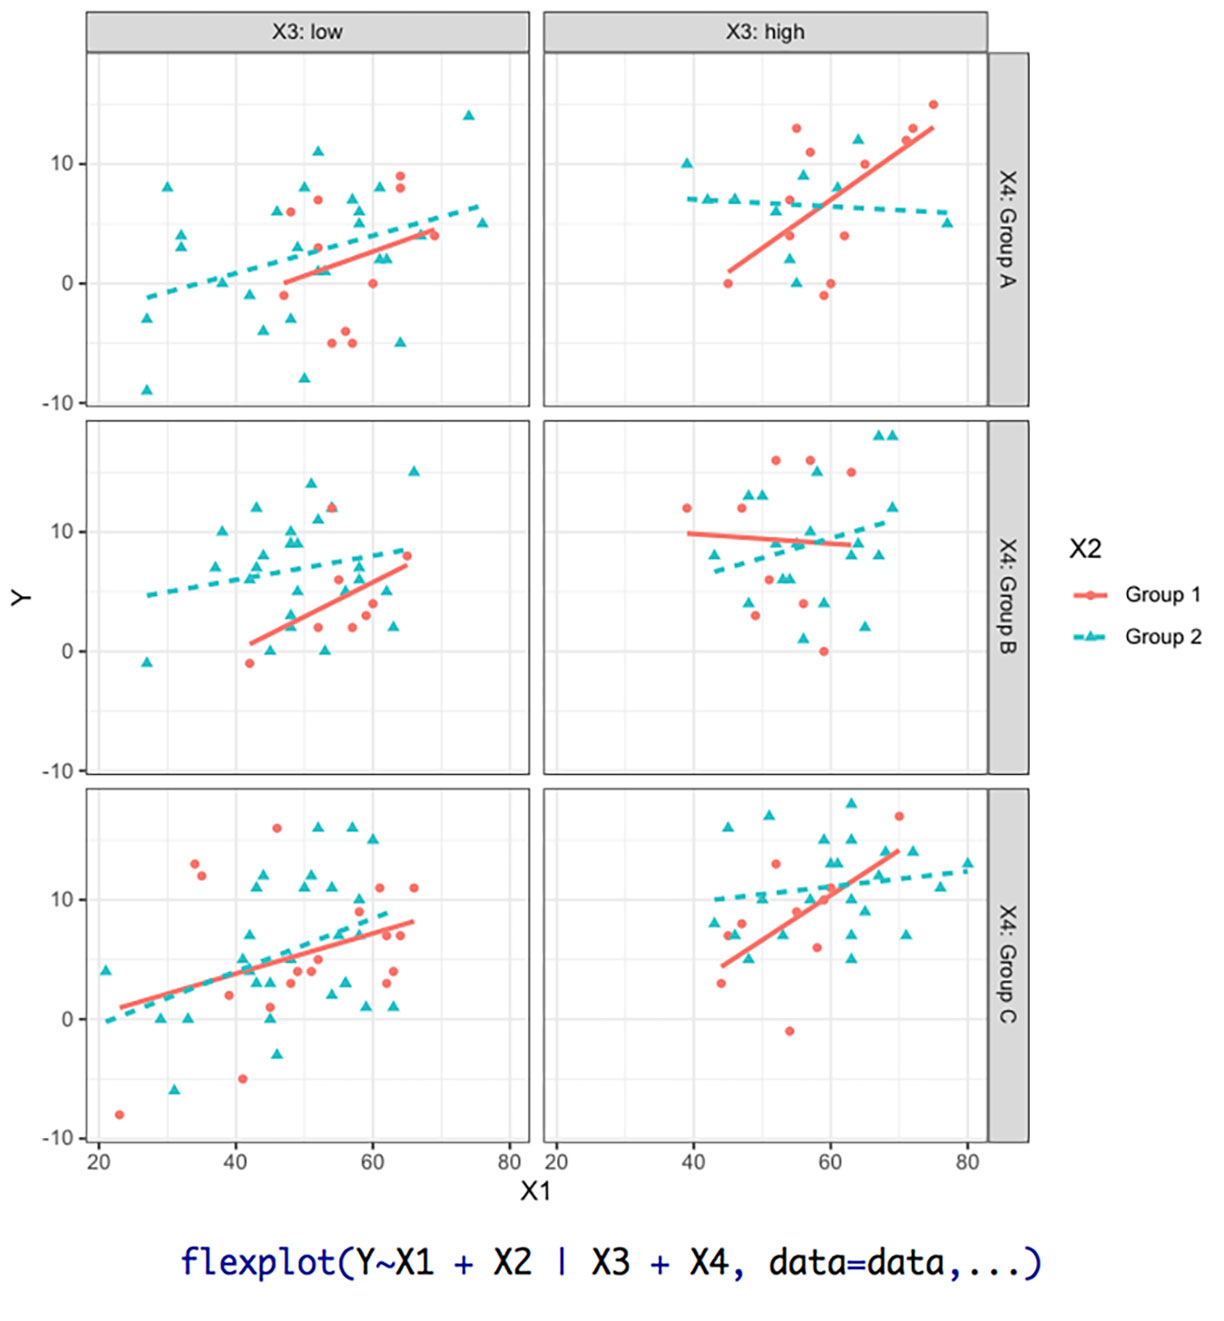
\includegraphics[width = 12cm]{images/flexplot_diagram.jpg} -->
<!-- \end{figure} -->
```{r, flexplotgrammar, out.width= "500px", fig.cap = "A diagram showing how elements of Flexplot's graphics are represented in a plot. $X1$ is shown on the $X$ axis, $X2$ shows up as different colors/symbols/lines, $X3$ panels in columns, and $X4$ panels in rows. \\label{fig:flexplotgrammar}", message=FALSE, warning=FALSE, echo=FALSE, fig.align='center'}
require(ggplot2)
require(flexplot)
data(exercise_data)
knitr::include_graphics("images/flexplot_diagram.jpg")
```



The base `plot()` function in \proglang{R} follows similar conventions as \pkg{flexplot} (i.e., users can specify an equation, such as `plot(y  ~  x)`), though `flexplot()` is more intelligent in its choice of displays. Also, `plot()` only allows the user to visualize one variable at a time. Another function, `coplot()`, allows some multivariate visualizations, yet it is limited in the types of data allowed and, like `plot()` is not flexible in the types of visualization decisions it makes. The \pkg{flexplot} package, on the other hand, offers great flexibility and automates much of the decision-making. 

In the following section, I will demonstrate how decisions are made in \pkg{flexplot}. I begin by showing how to produce univariate graphics, then bivariate graphics, then multivariate graphics. I will then follow that up with various functions and techniques for combining visuals with models, then conclude with a brief summary. 

# Univariate graphics

In `lm()`, one can fit an "intercept only" model, using the code `lm(y ~ 1)`. This is equivalent to estimating the mean of $y$. \pkg{flexplot} follows a similar convention with visualizing univariate distributions. However, the type of graphic displayed depends on the type of variable inputted into the function. For example, in the code below, notice that `flexplot()` recognizes whether the variable is categorical or numeric, and plots accordingly. 

```{r, message=FALSE, echo=TRUE, warning=FALSE, fig.cap = "A histogram (left) and barchart (right) produced within \\pkg{flexplot}.", fig.width = 6, fig.height = 3, out.width = "90%", fig.align = 'center'}
require(flexplot)
data(exercise_data) #### these are simulated data available 
                    #### in flexplot. Please don't base your 
                    #### weight loss program on this dataset
a = flexplot(weight.loss ~ 1, data = exercise_data)
b = flexplot(gender ~ 1, data = exercise_data)
cowplot::plot_grid(a , b)
```


Sometimes, `flexplot()` will make a wrong guess, if, for example, a categorical variable is recorded as a number (e.g., 1 = Group 1, 2 =  Group 2, 3  =  Group 3). To force `flexplot()` to produce a barchart, simply convert the variable to a factor (e.g., `data$group = factor(data$group, levels = 1:3, labels = c("Group1", "Group2", "Group3"))`). 

# Bivariate graphics

As with univariate graphics, \pkg{flexplot} will automatically produce an appropriate bivariate graphic, depending on the type of predictors and outcome variable: a numeric predictor/outcome will produce a scatterplot, a numeric predictor/categorical outcome = logistic curve graph, categorical predictor/numeric outcome = jittered density plot, and categorical predictor/categorical outcome = association plot. 

## Categorical predictor, numeric putcome (jittered-density plots)

There are many different ways to visualize a categorical predictor/numeric outcome relationship, including bar plots of means, box plots, violin plots, gradient plots, etc. Some are misleading (e.g., barplots of means and standard error plots). Others are mediocre (e.g., boxplots). Finally, some perform exceptionally well in human testing, including violin plots and gradient plots [@Correll2015]. `flexplot()` defaults to a "textured dot strip," which was invented by \cite{Tukey1990} \citep[see also][]{Wilkinson1999}. However, I am not too fond on the name. It lacks pizzazz. I have taken the liberty of renaming them "jittered density plots," or JD plots for short. I leave it to the reader to decide if this is pizzazzy enough. These are essentially violin plots with raw data. It is important to display raw data because without, it is impossible to tell the difference between a dataset with 15,000 versus 15 observations. For example, the two distributions in the left image in Figure \ref{fig:raw} look essentially the same, while the same data, plotted as JD plots, very clearly show the sample size. 

```{r, raw, message=FALSE, echo=TRUE, warning=FALSE, fig.cap = "Violin plots with 15,000 versus 15 datapoints. The outlines look the same in the left image, but the right image overlays the raw data, which makes the differing sample sizes much more apparent. \\label{fig:raw}", fig.width = 6, fig.height = 3, out.width = "90%", fig.align = 'center'}
group1 = c(0,1,2,2,3,3,3,3,3,3,4,4,5,6)
group2 = rnorm(10000,3,1)
d = data.frame(score = c(group1, group2), 
               group = c(rep("group 1", times = length(group1)), 
                       rep("group 2", times = length(group2))))
a = ggplot2::ggplot(data = d, aes(x = group, y = score)) +  
  geom_violin() + theme_bw()
b = flexplot(score ~ group, data = d)
cowplot::plot_grid(a, b)

```


In `flexplot()`, one can control the amount of jittering. The amount can be specified in multiple ways: as a boolean (`TRUE` means it will jitter, `FALSE` it will not), as a number (e.g., `0.2`), or as a vector (e.g., `c(.2, .4)`, which will indicate .2 jittering for X and .4 for Y). Just as it is in `geom_jitter()`, this number refers to the amount of jittering on either side. However, the value refers to the *maximum* amount the computer will jitter the data. So, 0.2 (the default) will jitter 10% of the way to the right only at the highest density and 10% to the left at the highest density. 

Users can also specify what the "whiskers" mean for the summary statistics. They default to the interquartile range (with the median as the center dot), but the user can also specify `sterr`, or `stdev,` to indicate the standard error or standard deviation:


```{r, jitterit, message=FALSE, echo=TRUE, warning=FALSE, fig.cap = "Dot plots with the interquartile range and no jittering (left), JD plot with mean + standard errors and jittering on $X$ and $Y$ (middle), and JD plot with mean + standard deviation with jittering on only $X$ (right).", fig.width = 6, fig.height = 2.5, out.width = "90%", fig.align = 'center'}
a = flexplot(weight.loss ~ therapy.type, data = exercise_data, 
             jitter = F, spread = "quartile")
b = flexplot(weight.loss ~ therapy.type, data = exercise_data, 
             jitter = c(.4,.5), spread = "sterr")
c = flexplot(weight.loss ~ therapy.type, data = exercise_data, 
             jitter = .2, spread = "stdev")
cowplot::plot_grid(a, b, c, nrow = 1)
```


## Numeric predictor, numeric outcome (scatterplots)

The indisputed king of numeric on numeric visualization is the scatterplot. Once again, `flexplot()` is smart enough to choose a scatterplot when it is passed a numeric predictor and numeric outcome. The fit of the graph defaults to a loess line, so as to highlight deviations from linearity. However, the user can specify other sorts of fits, such as `"lm"` (for regression), `"polynomial"`, `"cubic"`, and `"rlm"` (robust linear model) in the \pkg{MASS} package [@mass]. The user can also choose to remove the confidence interval by specifying `se = F`, as well as jitter one or both variables, as shown below. 

```{r, message=FALSE, echo=TRUE, warning=FALSE, fig.cap = "Scatterplot with different options of fit: \\code{loess} (default), \\code{lm} (regression), \\code{polynomial}. Also, the data in the far right plot has been jittered. ", fig.width = 6, fig.height = 2.5, out.width = "90%", fig.align = 'center'}
a = flexplot(weight.loss ~ satisfaction, data = exercise_data) + 
  theme_minimal() ### using layering to change theme
b = flexplot(weight.loss ~ satisfaction, data = exercise_data, 
             method = "lm", se = F)
c = flexplot(weight.loss ~ satisfaction, data = exercise_data, 
             method = "polynomial", jitter = .4)
cowplot::plot_grid(a, b, c, nrow = 1)
```


## Numeric predictor, categorical outcome (logistic curves)

`flexplot()` also has some ability to model categorical outcomes. One common situation might be when one is attempting to model a binary outcome, as they would in a logistic regression. Any binary variable can be visualized as a logistic regression in \pkg{flexplot}, except when the axis variable is also categorical (i.e., the variable occupying the first slot in the `flexplot()` equation, which in the case of Figure \ref{fig:logistic} is `attention`). To do so, the user only needs to specify `logistic` as the method. 

```{r, logistic, message=FALSE, echo=TRUE, warning=FALSE, fig.cap = "Example of a logistic plot in the \\pkg{flexplot} package.\\label{fig:logistic}", out.width="40%", fig.width = 3, fig.height = 3}
data("tablesaw.injury") ### also simulated data available 
                        ### in flexplot package
                        ### always remember to be safe 
                        ### and attentive when woodworking
flexplot(injury ~ attention, data = tablesaw.injury, 
             method = "logistic", jitter = c(0, .05))
```

## Categorical outcome, categorical predictor (association plots)

Sometimes the analyst may wish to visualize the relationship between two categorical variables. Once again, `flexplot()` is smart enough to determine that information from the formula, provided the user supplies two factors. In this situation, `flexplot()` will generate an "association" plot, which plots the deviation of each cell from its expected frequencies (divided by the expected values within that cell). In the example below, I had to convert `injury` to a factor to get a barplot. The graphic (Figure \ref{fig:association}) shows that females are less likely to be injured than males, relatively speaking. 

```{r, association, message=FALSE, echo=TRUE, warning=FALSE, fig.cap = "Example of an association plot for categorical predictor/categorical outcome.\\label{fig:association}" , out.width="40%", fig.width = 3.5, fig.height = 2.5}
tablesaw.injury$injury = factor(tablesaw.injury$injury, 
                  levels=c(0, 1), labels=c("all good", "ouch"))
flexplot(injury ~ gender, data = tablesaw.injury)

```


## Repeated measures data (related t-test)

As I mentioned previously, one of the guiding tenets of \pkg{flexplot} is that every statistical analysis ought to be accompanied by a graphic that closely matches the analysis. With a related t-test, the existing graphics will not accurately represent this model because a related $t$ actually models the *difference* between scores (e.g., from Time 1 to Time 2). As such, `flexplot()` allows an additional option (`related = TRUE`) that tells `flexplot()` to plot the differences, rather than the groups. To do so, `flexplot()` requires "tidy" data [@tidy], or data where Time is indicated in one column and the score in the other. Also, there must be equal numbers of observations in each group. Once in this format, it simply plots the differences (Figure \ref{fig:plant}). For example:

```{r, plant, message=FALSE, echo=TRUE, warning=FALSE,out.width="40%", fig.width = 3, fig.height = 3, fig.cap = "A plot of repeated measures data.\\label{fig:plant}"}
data("plant_growth")
flexplot(Diameter ~ Soil.Type, data = plant_growth, related=T)
```

\noindent (Note, this dataset didn't actually contain repeated measures data. This is merely for illustrative purposes). 

Unfortunately, plotting difference scores only works with two timepoints. When there are more than two timepoints, I recommend visualizing these relationships with the `visualize()` function using mixed models. (I'll address `visualize()` shortly). In the plant growth graphic, the differences seem centered around zero, indicating that the type of potting soil used (store-bought potting soil versus a "secret" custom mix I found online) didn't make a difference in seedling diameter. 

## Avoiding overlap

If it wasn't yet apparent, let me be less subtle: I think all graphics should include raw data. Showing raw data allows readers to determine whether the chosen model is appropriate, and it communicates the degree of uncertainty about the model. However, when there are a large number of datapoints, it becomes quite difficult to see any patterns; areas of high density look just as crowded as areas of lower density, relatively speaking (although having JD plots makes it clear which areas are most dense; see the example in top-left image in Figure \ref{fig:sample}). To address such overlap, `flexplot()` offers three options. The first is to suppress raw data (`raw.data = F`, right-top in Figure \ref{fig:sample}). I don't recommend that, but it can be done. A second option is to reduce the transparency (e.g., bottom-left in Figure \ref{fig:sample}). Perhaps the best option is to *sample* (bottom-right in Figure \ref{fig:sample}). However, it is important that the visual display of fit (e.g., median + IQR, loess line, regression line) not be estimated from the sampled data. Rather, the fit should correspond to the entire dataset. `flexplot()` performs this operation in the background. In Figure \ref{fig:sample}, notice how the medians/interquartile ranges do not change, despite having different numbers of datapoints. 

```{r, sample, message=FALSE, echo=TRUE, warning=FALSE, fig.cap = "Four graphics showing different ways to handle overlapping datapoints. The top-left image does nothing. The top-right does omits raw data. The bottom-left reduces the opacity of the points. The bottom-right samples datapoints. \\label{fig:sample}"}
data("nsduh")
a = flexplot(distress ~ major.dep, data = nsduh)
b = flexplot(distress ~ major.dep, data = nsduh, raw.data = F)
c = flexplot(distress ~ major.dep, data = nsduh, alpha = .005)
d = flexplot(distress ~ major.dep, data = nsduh, sample = 200)
cowplot::plot_grid(a, b, c, d, nrow = 2)
```


# Multivariate graphics

Visualizing multivariate relationships can become quite tricky. It is very easy to induce cognitive overload, especially when attempting to visualize raw data (which is, again, a key characteristic of \pkg{flexplot}). Some might be inclined to create three-dimensional plots. However, these are difficult to interpret and they require the user to rotate the view. Even then, they can only show two predictors at a time. I find it much easier to use other strategies. `flexplot()` utilizes four different strategies to visualize multivariate relationships: (1) plotting a dimension as different colors/lines/shapes, (2) plotting a dimension in row or column panels, (3) visualizing conditional relationships with added variable plots, and (4) overlaying ghost lines. 

\subsection[Added variable plots (AVPs) with added.plot()]{Added variable plots (AVPs) with \code{added.plot()}} \label{sec:added.plot}

AVPs are underused, yet extremely useful. Essentially, an AVP shows the relationship between a predictor of interest and the *residuals* of an existing model. For example, if one wanted to understand the relationship between `therapy.type` and `weight.loss` after controlling for motivation, that person could build a model predicting \code{weight.loss} from \code{motivation}, residualize that relationship, then show a JD plot of the residuals for each type of therapy. This is what AVPs do (see Figure \ref{fig:avp}). \pkg{flexplot}'s version of AVPs have a slightly different flavor. In my experience, AVPs can be confusing to lay audiences because the scale of the outcome variable has changed to be centered on zero. To counter this confusing, \pkg{flexplot} adds the mean back into the residuals so the $Y$-axis retains the original scale. The notation for `added.plot()` is similar to `flexplot()`, though the vertical pipes aren't necessary. What `flexplot()` will do is take the *last* variable entered (`therapy.type` in the following example) and plot that on the $X$ axis, while plotting the residuals of the model on the $Y$ axis (i.e., the residuals of the model `weight.loss ~ motivation`). Other arguments can be passed to `added.plots()` as well (such as `alpha`, `sample`, `method`, etc.)

```{r, avp, message=FALSE, echo=TRUE, warning=FALSE, fig.width = 3, fig.height = 2, out.width = "50%", fig.cap = "An Added Variable Plot (AVP) showing the relationship between \\code{therapy.type} and \\code{weight.loss}, after controlling for \\code{motivation}. \\label{fig:avp}"}
added.plot(weight.loss ~ motivation + therapy.type, data = exercise_data)
```

## Colors/lines/shapes

As shown in Figure \ref{fig:flexplotgrammar}, the second slot in the `flexplot()` formula (`X2` in Figure \ref{fig:flexplotgrammar}) controls which variable is displayed as different colors/symbols/lines. Figure \ref{fig:symbols} shows two examples of this: one where a numeric predictor is on the $X$ axis, and one where a categorical predictor is on the X-axis. When categorical variables are shown on the X-axis, `flexplot()` draws lines connecting the medians (or means). 

```{r, symbols, message=FALSE, echo=TRUE, warning=FALSE, fig.width = 6, fig.height = 3, out.width = "90%", fig.align = 'center', fig.cap = "Two multivariate graphs illustrating how the second slot in a \\pkg{flexplot} formula controls the visualization. The left image demonstrates what happens to the second slot variable ($X2$) when a numeric predictor is on the X-axis, while the right image demonstrates what happens to the second slot variable when a categorical predictor is on the X-axis.\\label{fig:symbols}"}
a = flexplot(weight.loss ~ motivation + gender, 
    data = exercise_data, se = F, alpha = .3)
b = flexplot(weight.loss ~ therapy.type + gender, 
    data = exercise_data, se = F, alpha = .3)
cowplot::plot_grid(a, b)
```
One limitation of colors/shapes/symbols is the increase in cognitive load. When plotting different symbols/colors/lines on the same graph, there is often a great deal of overlap, which makes it more difficult to pick out patterns. In my experience, having a variable with more than two levels in the second slot of a `flexplot()` equation becomes challenging to interpret, particularly when there are more than a handful of datapoints. 

## Paneling

An alternative (or additional) strategy for plotting multivariate data is paneling. As shown in Figure \ref{fig:flexplotgrammar}, the third and fourth slots control paneling in columns and rows, respectively. The panels follow many conventions developed by William Cleveland [-@Cleveland1994], such as having values increase from left to right and bottom to top (just as they do on the $X$ and $Y$ axis, respectively). 

Figure \ref{fig:panels} shows the same relationships in Figure \ref{fig:symbols}, but with the second variable in panels instead. The bottom image also displays panels for three variables simultaneously. Paneled variables are easy to conceptualize with categorical variables, but what about numeric variables? These can still be visualized, but the values must be binned. Also notice that I have taken advantage of the fact that `flexplot()` returns a \pkg{ggplot2} object that can be edited. In this case, I am both layering (modifying the behavior of the labels to prevent cutting them off) and modifying the \pkg{ggplot2} object itself (reducing the size of the points in the final graphic).[^foot]

[^foot]: I also do not show the code where I actually plot the graphics. This required some advanced manipulation of the layout and I didn't want to detract from what `flexplot()` is doing. 

```{r, message=FALSE, echo=TRUE, warning=FALSE}
a = flexplot(weight.loss ~ motivation | gender, 
             data = exercise_data)
b = flexplot(weight.loss ~ therapy.type | gender, 
             data = exercise_data)
c = flexplot(weight.loss ~ motivation |  gender + therapy.type, 
             data = exercise_data) +
      ggplot2::facet_grid(therapy.type ~ gender, 
              labeller = ggplot2::labeller(therapy.type = label_value)) 
#### edit point size
c = ggplot2::ggplot_build(c)
c$data[[1]]$size = .25
c = ggplot2::ggplot_gtable(c)

```


```{r, panels, message=FALSE, echo=FALSE, warning=FALSE, fig.align = "center", out.width = "90%", fig.cap = "A multivariate plot where \\code{therapy.type} and \\code{gender} are now shown in panels. \\label{fig:panels}", fig.width = 5, fig.height = 5}
		top.row = cowplot::plot_grid(a, b, ncol = 2)
		bottom.row = cowplot::plot_grid(NULL, c, NULL, ncol = 3, rel_widths=c(.25, .5, .25))
		cowplot::plot_grid(top.row, bottom.row, nrow = 2, rel_heights=c(.55, .45))
  
```



## Binning

Within `flexplot()`, any numeric predictor, with the exception of the variable in the first slot, will be binned into discrete categories. These bins will then be represented in panels (if the variable is in the third or fourth slot) or as colors/symbols/lines (if the variable is in the second slot). The user has the option of specifying the number of bins (e.g., 2 or 3), or the user can specify breakpoints at which to bin. When the user specifies bins, `flexplot()` will attempt to have an equal number of datapoints in each bin. However, `flexplot()` may be unable to bin into the specified number of bins. For example, if a user specifies four bins, it is possible the scores at the 50th and 75th percentile are the same. In these cases, `flexplot()` will choose a smaller bin number, though it will report such to the user. `flexplot()` defaults to three bins. 

When specifying breakpoints, the panels may have different sample sizes in each bin. A user may wish to do this if these breakpoints are meaningful (e.g., when particular scores are clinically meaningful, such as Beck Depression Inventory scores above 29 are considered severly depressed). 

Whether using breakpoints or bins, the user can also specify labels for the bins. Figure \ref{fig:panels2} shows three plots of the same variables: the first specifies two breakpoints, the second specifies breakpoints with labels, and the third just specifies the number of bins. 

```{r, message=FALSE, echo=TRUE, warning=FALSE}
a = flexplot(weight.loss ~ motivation | satisfaction, 
             data = exercise_data, 
             breaks = list(satisfaction=c(3,7))) +
  ggplot2::facet_grid( ~ therapy.type, 
              labeller = ggplot2::labeller(therapy.type = label_value))
b = flexplot(weight.loss ~ motivation + satisfaction, 
             data = exercise_data, 
             breaks = list(satisfaction=c(3,7)), 
             labels = list(satisfaction=c("low", "medium", "high")))
c = flexplot(weight.loss ~ motivation + satisfaction, 
             data = exercise_data, 
             bins = 2) 

```

```{r, panels2, fig.align = "center", out.width = "90%",fig.height = 6, fig.width = 8,  fig.cap = "Plots reflecting choices of different break points (left-most plot), labels (right plot), and bins (bottom plot). \\label{fig:panels2}",message=FALSE, echo=FALSE, warning=FALSE}
  top.row = cowplot::plot_grid(a, b, ncol = 2, rel_widths=c(1,1.5))
  bottom.row = cowplot::plot_grid(NULL, c, NULL, ncol = 3, rel_widths=c(.2, .6,.2))
  cowplot::plot_grid(top.row, bottom.row, nrow = 2,rel_heights = c(.55, .45))
```


## Ghost lines

There are advantages and disadvantages to plotting a variable as a color/symbol/line versus panels. Panels reduce clutter, but make it harder to make comparisons because the eye has to travel further to make such comparisons. On the other hand, plotting in the same panel with different colors/lines/symbols means less visual distances to travel, but then there is too much clutter. One obvious solution is to stick with colors/symbols/lines and reduce transparency (or sample). However, there is a more innovative way of resolving this difficulty, by using something I call ghost lines. Ghost lines repeat the relationship from one panel to the other panels to make it easier to compare. Figure \ref{fig:ghost} demonstrates how to use ghost lines. By default, `flexplot()` chooses the middle panel for odd numbers of panels, otherwise it chooses a panel close to the middle. The second line of code below specifies the referent panel by picking a value in the range of the referent panel. In Figure \ref{fig:ghost}, the ghost lines makes it clear that the relationship between `motivation` and `weight.loss` is stronger both at low and high levels of `satisfaction`, but less so at medium levels. 

```{r, ghost, message=FALSE, echo=TRUE, warning=FALSE, fig.cap = "Ghost lines repeat the pattern from one panel to the others, making it easier to compare across panels. \\label{fig:ghost}", out.width = "80%", fig.width = 5, fig.height = 3, fig.align = 'center'}
flexplot(weight.loss ~ motivation | satisfaction, 
             data = exercise_data, method = "lm", 
             bins = 3, ghost.line = "red")
```


## General strategy for plotting multivariate relationships
It is easy for multivariate visuals to become unnecessarily complicated. For example, the top image in Figure \ref{fig:threeway} shows a graphic where all four `flexplot()` slots are occupied. This is very difficult to interpret what is going on. To simplify things, we could utilize several strategies. First, we can specify two bins instead of the default three. We can also remove confidence intervals, reduce the opacity of the data, and plot regression lines.[^foot2] Also, I generally try to have only two levels for the variable in the second slot (in this case, Male versus Female). Finally, we could add ghost lines. The bottom image in Figure \ref{fig:threeway} utilizes all these strategies and simplifies the visual interpretation immensely.

[^foot2]: These are great strategies to use *after* one has determined that the model generally fits the data. If the data are curvilinear, for example, it would not make sense to plot straight lines or make the datapoints overly transparent. 

Another strategy is to mentally block out all panels but the diagonal (the bottom-left to top-right). The diagonal reflects the influence of *both* variables as they increase (or decrease). In other words, they are a rough approximation of the average effect of the $X1/Y$ relationship as you increase (or decrease) the paneled variables. If there is a general pattern of the lines consistently getting steeper (or shallower) as they move up the diagonal, that indicates there may be a three-way interaction effect. In Figure \ref{fig:threeway}, the lines seem pretty parallel going from bottom-left to top-right. The one thing that *does* seem to change is that the colored lines go from below the ghost line to above it (indicating a main effect of `health` and/or `satisfaction`). In other words, we may be safe to do AVPs. However, before doing so, it may be best to combine visuals with statistical modeling.

```{r, threeway, message=FALSE, echo=TRUE, warning=FALSE, fig.cap = "Multivariate relationship between five variables. Each \\pkg{flexplot} slot is occupied and it is difficult to interpret what is going on in the top figure, though the use of regression lines instead of loess lines, removing standard errors, reducing transparency of the datapoints, adding ghost lines, and reducing the number of bins have made it  easier to interpret (bottom image).  \\label{fig:threeway}", fig.width = 6, fig.height = 8}


a = flexplot(weight.loss ~ motivation + gender | satisfaction + health, 
    data = exercise_data) 
b = flexplot(weight.loss ~ motivation + gender | satisfaction + health, 
    data = exercise_data, 
    method = "lm", se = F, bins = 2, ghost.line = "black", alpha = .2,
    ghost.reference = list(satisfaction = 0, health = 10, gender = "male"))
cowplot::plot_grid(a, b, ncol = 1)
```


# Combining modeling and visualizations
Visuals are great for conveying general trends and patterns. However, it can be difficult to make decisions based on graphics, particularly when the pattern is not striking. For example, in Figure \ref{fig:threeway}, I don't feel entirely comfortable rejecting the idea that there are no interactions present in the model. Statistics, on the other hand, put visual patterns into concrete numbers that assist with statistical decision-making. Furthermore, it is easy to engage in confirmation bias when viewing a graphic. Statistics provide a much-needed reality check. As such, the two, statistics and visualizations, ought to proceed hand in hand. Fortunately, \pkg{flexplot} was designed to complement statistical analysis (and vice versa). More specifically, \pkg{flexplot} has two additional visualization functions that simplify modeling, as well as two functions dedicated to statistical analysis. 

\subsection[The visualize() function]{The \code{visualize()} function} \label{sec:visualize}
As I've mentioned repeatedly, one of the primary purposes of \pkg{flexplot} is provide visualization for statistical models. The `visualize()` function is designed to do exactly that. Much like `summary()`, or `coef()`, `visualize()` is an R method within \pkg{flexplot} that can be applied to diverse sorts of models, including `lmer`, \code{lm}, and `glm`. `visualize()` attempts to generate a graphic that matches the formula used in a fitted model. Not only will `visualize()` plot a graphic to match the analysis, but it will also show diagnostic plots. For example, if we were to fit an ANCOVA model, we could visualize it as follows:

```{r, ancova, message=FALSE, echo=TRUE, warning=FALSE, fig.cap = "Demonstration of the \\code{visualize} function on a \\code{lm} object. The top row shows two different representations of the statistical model. The bottom row shows diagnostic plots.  \\label{fig:ancova}", out.width = '80%', fig.width=8, fig.height=8}

model = lm(weight.loss ~ motivation + therapy.type, 
           data = exercise_data)
visualize(model)
```

For multivariate data, visualize will default to producing two graphics to match the analysis: one AVP (top right graphics in Figure \ref{fig:ancova}) and one other plot that will use panels and/or colors/symbols/lines. It will also generate diagnostic plots (histogram of the residuals, residual dependence plots, and S-L plots). The user can specify *just* a plot of the model (`visualize(model1, "model")`), or *just* a plot of the diagnostics (`visualize(model1, "residuals")`). Additionally, visualize can take `flexplot()` arguments and even a `flexplot()` formula.

```{r, ancova2, message=FALSE, echo=TRUE, warning=FALSE, fig.cap = "Demonstration of the visualize function on a \\code{lm} object, but with \\pkg{flexplot} arguments controlling the output (as well as suppressing residuals).  \\label{fig:ancova2}"}
model = lm(weight.loss ~ motivation + therapy.type, data = exercise_data)
visualize(model, formula = weight.loss ~ motivation | therapy.type, 
          ghost.line = "red", se = F, method = "lm", plot = "model")
```

Figure \ref{fig:mixed} shows the `visualize()` function for a mixed model. With mixed models, `visualize()` randomly samples from the random effects (`Subject` in this case) and plots that as a variable in the graphic, and its location on the graph depends on whether the user specifies `formula`. If they do not, `visualize()` will default to placing it in the second slot (different lines/colors/shapes). This allows the user to visualize a subset of the subjects in a mixed model to ensure the model chosen is appropriate. 

```{r, mixed, message=FALSE, echo=TRUE, warning=FALSE, fig.cap = "Demonstration of the \\code{visualize} function for a mixed model. In this graphic, each dashed line represents the fit of a particular school. \\label{fig:mixed}"}
require(lme4)
data(math)
model = lmer(MathAch ~ Sex + SES + (SES|School), data = math)
visualize(model, 
  plot = "model",
  formula = MathAch ~  Sex + School| SES, 
  sample = 30)
```

\subsection[The compare.fits() function]{The \code{compare.fits()} function} \label{sec:compare.fits}

Very often in statistical modeling, we are interested in comparing two models, such as one with and one without an interaction term. There are many statistics available that allow easy comparison between models, such as the AIC, BIC, Bayes Factor, $R^2$, p-values, etc. However, it is again important to *see* how the two models differ in terms of fit. On multiple occasions, I have found various statistics show preference for one model, yet the visuals show the two models differ in only trivial ways. 

That is where `compare.fits()` comes in. It is simply a wrapper for the `predict()` function, combined with the graphing capabilities of \pkg{flexplot}. More specifically, `compare.fits()` will overlay the fit of both models onto the raw data. For example, Figure \ref{fig:compare} shows the fit of two different models, one that includes an interaction and the other that does not. The arguments are very similar to `flexplot()`, but with the addition of the model objects. Likewise, `compare.fits()` takes many of the same arguments. In this example, I've overlaid a black ghost line. Notice that the two lines (from `lm` and `interaction`) generate very similar predictions across the range of data, suggesting that a main effects model may be sufficient. 

```{r, compare, message=FALSE, echo=TRUE, warning=FALSE, fig.cap = "Demonstration of the \\code{compare.fits()} function, comparing a main effects and an interaction model. Ghost lines have been added from the \\code{cog} condition for easier comparison across panels. \\label{fig:compare}", fig.width = 5, fig.height = 3.5}
model.me = lm(weight.loss ~ motivation + therapy.type, data = exercise_data)
model.int = lm(weight.loss ~ motivation * therapy.type, data = exercise_data)
compare.fits(weight.loss ~ motivation | therapy.type, 
             data = exercise_data, model.me, model.int, ghost.line = "black")+
      ggplot2::facet_grid( ~ therapy.type, 
          labeller = ggplot2::labeller(therapy.type = label_value))
```

# Functions devoted to estimation

The \pkg{flexplot} package specializes in visualization, providing easy-to-use tools for graphical data analysis. However, it also has a small collection of non-visual functions that can be used hand-in hand with visuals. These functions include the `estimates()` method and `model.comparison()`. 

\subsection[The estimates() Function]{The \code{estimates()} function} \label{sec:estimates}

The `estimates()` function was designed to report paremeter estimates and effect sizes. Much like `flexplot()`, many of the decisions are made in the background. And like `visualize()`, `estimates()` takes a fitted object as input. `estimates()` will then determine which estimates are most appropriate. For grouping variables, `estimates()` will report means, mean differences, and cohen's $d$, as well as 95% confidence intervals. For numeric variables, `estimates()` will report the intercept, slopes, and standardized slopes, also with corresponding confidence intervals. Additionally, it will report the model $R^2$, as well as the semi-partial $R^2$ associated with each effect in the model, except when there are interactions in the model. (With interactions present, it does not make sense to interpret main effects, which is why `estimates()` only reports the semi-partial for the interaction effect).  

```{r, message=FALSE, echo=TRUE, warning=FALSE}
estimates(model.int)
```
The estimates shown support the conclusions gleaned from Figures \ref{fig:ancova}-\ref{fig:ancova2}, as well as Figure \ref{fig:compare}, namely that the addition of the interaction likely is not improving the fit enough to consider keeping. 

\subsection[The model.comparison() Function]{The \code{model.comparison()} Function} \label{sec:model.comparison}

The final function I will mention is the `model.comparison()` function. This is similar to the `anova()` function in base \proglang{R}, but it includes additional estimates, including AIC, BIC, and the BIC-derived Bayes Factor. Additionally, `model.comparison()` works on both nested and non-nested functions. When used on non-nested functions, it will only compute AIC, BIC, and Bayes Factor. Also, the `model.comparison()` function will report the quantiles of the *differences* in prediction, in standardized units. The `model.comparison()` below compares the main effects and the interaction model. The last reported numbers indicate that the maximum difference in prediction between the two models is only about a third of a standard deviation, while the median difference is only about 0.05 standard deviations, suggesting the predictions are quite similar. Also, all statistics (AIC, BIC, Bayes Factor, p-value, and probably $R^2$) support the more simplified main effects model. 

```{r, message=FALSE, echo=TRUE, warning=FALSE}
model.comparison(model.int, model.me)
```

# Summary

This paper has sought to demonstrate the utility of the \pkg{flexplot} package. This visual approach to data analysis has many advantages, including emphasizing uncertainty, improving encoding, and increasing communication with lay audiences. The formula-based, layered grammar of graphics makes many basic and advanced plotting functions much easier to produce, and does so using scientifically-derived principals of human perception. Additionally, \pkg{flexplot} allows tools that permit seamless integration of statistical analysis with visual interpretation.

# Computational details

All analyses were conducted in \proglang{RStudio} [@RStudioTeam2016], version 1.1.463. Styling was produced with \proglang{RMarkdown} [@Xie2018], v 1.16 and \proglang{rticles} [@Allaire], v 0.11.1. This document used \pkg{flexplot} version 0.6.2, which is available at http://www.github.com/dustinfife/flexplot. Modifications to the displayed graphics were created using \proglang{ggplot2} 3.2.1.9000 [@Wickham2011b] and \pkg{cowplot} [@Wilke2016]. Mixed models were fit using \pkg{lme4} [@lme4].  

